\documentclass[12pt, letterpaper]{article}
\usepackage[margin=0.8in]{geometry}
\usepackage[utf8]{inputenc}
\usepackage[super,comma]{natbib}
\usepackage{graphicx}
\usepackage{xcolor}

\usepackage{hyperref}

\title{CMSC499A: Mutation Signature Explorer}
\author{Mark Keller \thanks{advised by Professor Max Leiserson}}
\date{Spring 2018}

\begin{document}
\maketitle

\begin{abstract}
Identification and analysis of patterns in data can be difficult without visualization tools. 
Datasets of somatic mutations in cancer are no exception.
Recent whole-genome sequencing projects have produced large amounts of mutation data to be explored.
Of great importance is the classification of different mutational processes and the mutational signatures\cite{alexandrov2013signatures} they leave behind.
As new mutational signatures continue to be discovered, observation of the levels of signature activity, called signature exposure, helps show how the underlying mutational processes differ across cancer types, time, and environmental variables.
This paper describes a mutation visualization tool developed this semester that allows simple somatic mutation datasets and mutation signatures to be explored interactively and provides users with publication-ready graphics.
\end{abstract}

\section{Introduction}
Mutation Signature Explorer is a web-based (\url{https://mutation-signature-explorer.lrgr.io}) mutation data browser that enables exploration of mutational signatures, single-nucleotide variant (SNV) mutations, and mutation density.
This tool allows users to choose sequencing project datasets by cancer type, as well as mutational signature combinations (of which can be selected based on cancer-type-specific presets) before plotting this data. 
Web-based interactive visualizations allow for exploration across datasets and features in a way that is accessible and fast.
Data exploration through these visualizations can be used to make initial inferences that lead to further statistical analysis, or, alternatively, can be used to verify and communicate relationships found through prior analysis.

Each type of visualization produced by the Mutation Signature Explorer aims to enable further examination of a trend or relationship which has been hypothesized or presented in existing literature.
The following are types of visualizations that can be generated and their motivations:
\begin{enumerate}
\item It is well known that tobacco and alcohol usage increases risk of many types of cancers \cite{doll1956lung,collaborative2002alcohol}. A question of interest is how mutational signatures relate to smoking status and other clinical variables. Alexandrov \textit{et al}. 2016 finds that smokers exhibit increases in mutations attributed to COSMIC signatures 2, 4, 5, 13, and 16 \cite{alexandrov2016mutational}. Kim \textit{et al}. 2016 also notes an association between signature 5 and smoking \cite{kim2016somatic}.

To illustrate estimated contributions of a selected combination of mutational signatures, a stacked bar plot can be generated, showing estimated signature exposures for a sample, along with tobacco and alcohol usage indicators.
Exposure values can be normalized to sum to one for each sample, or kept relative to the total number of mutations in each sample.
This plot type was inspired by Figure 4 in Kim \textit{et al.} 2016 that displays estimated contributions of 4 different signatures and tobacco usage over cohorts of urothelial cancer tumor samples \cite{kim2016somatic}.
    
\item Localized hypermutation, known as kataegis, was first discussed by Taylor \textit{et al}. 2013\cite{taylor2013dna}, in which whole-genome sequencing of breast cancers showed regions with mutation ``rainfalls" - greater than 5 mutations with significantly short intermutational distances. Mutations in regions of kataegis have been shown to occur frequently at C base pairs preceded by a 5-prime T base pair, due to APOBEC activity during double-strand break repair\cite{taylor2013dna}. Since this introduction in 2013, kataegis has been shown to occur in additional tumor types\cite{alexandrov2013signatures}. COSMIC signatures 2 and 13 have been associated with APOBEC activity, and by extension, kataegis\cite{alexandrov2013signatures}. There is recent interest in rigorous statistical identification and verification of kataegis\cite{yousif2018origins}.

To examine mutation clusters, specifically those occurring in regions of kataegis, a rainfall plot can be generated for each sample.
Mutations are plotted horizontally based on their genome location, and vertically by the distance (in bp) to the previous mutation.
Mutations are colored according to one of 96 mutation categories (5' flanking base pair, single-nucleotide variant, 3' flanking base pair).
Rainfall plots are commonly used to examine regions of hypermutation, as they allow these regions to be easily identified by tight vertical clusters of mutations. 
Similar rainfall plots can be seen in Figure 4 of Nik-Zainal \textit{et al.} 2012\cite{nik2012mutational} and in Figure 6 of Alexandrov \textit{et al}. 2013\cite{alexandrov2013signatures}.

To identify samples containing instances of localized hypermutation kataegic events can be highlighted along the genome in a second type of plot.
Along the vertical axis are samples, and along the horizontal axis is the genome.
Users can zoom and pan along each chromosome, and easily pinpoint kataegis events by the dark bars located on mutations in kataegis regions.
Samples are grouped by sequencing project and cancer type.
This plot acts as a rainfall plot selector, as each sample bar can be clicked to generate a corresponding rainfall plot.
To our knowledge, this style of plot has not been used before to visualize kataegis .
    
\item A question that prompted the development of this visualization tool is whether certain mutational signatures are associated with mutations in specific genomic locations or regions.
One way to examine this is to look at mutation signature activity across the genome with a ``Manhattan plot".
The Manhattan plot gets its name from the resemblance of a skyline along the genome, and is typically used to visualize genome-wide association studies\cite{gibson2010hints}.
To generate this plot, signatures are assigned to individual mutations and then grouped into bins by chromosome location and signature.
A signature is assigned to each mutation category (5' flanking base pair, single-nucleotide variant, 3' flanking base pair) for each sample by first computing estimated signature exposures for a sample, then taking the maximum of the product of each signature's probability for the mutation category and the sample's exposure to the same signature.
The horizontal axis represents the genome location, and the vertical axis represents the number of mutations within a bin.
To our knowledge, this is a new method for exploring mutational signatures along the genome.

\end{enumerate}


\section{Case Study}

\subsection{Alcohol Usage and Mutational Signatures}
One use case for this tool is the analysis of relationships between signature exposures and clinical variables.
Interactive sorting and dynamic calculations of signature exposures allow trends to be observed quickly.
Although the relationship between liver cancer and alcohol consumption has long been documented \cite{bosch2004primary}, the relationship between mutational signatures and alcohol consumption has not been extensively examined.
Recently, Li \textit{et al}. 2018 identified a mutational signature associated with alcohol usage in esophageal squamous cell carcinoma that resembles COSMIC signatures 1, 2, 13 and 16\cite{li2018mutational}.
To look for a relationship in liver cancer with the Mutation Signature Explorer, we can select the PCAWG Liver Cancer - NCC, JP cohort, along with the COSMIC LICA signatures preset for liver cancer. 
Then, to examine the alcohol usage clinical variable, we can select the Signature Exposures with Clinical Data plot.
Using the sorting functionality, we first sort by the alcohol usage clinical variable.
With no trends immediately apparent, we can now sort by signature values.
Sorting by COSMIC signature 12 and normalizing the signature exposures, we can see that only two alcohol-free donors are in the top 14 of 28 donors (Figure \ref{fig:caseStudy1_sig12}).
\begin{figure}[h]
    \centering
    \frame{\includegraphics[width=0.75\columnwidth]{figures/case_study1.png}}
    \caption{Screenshot of Signature Exposures with Clinical Data plot with PCAWG-LINC-JP data, normalized and sorted by COSMIC signature 12}
    \label{fig:caseStudy1_sig12}
\end{figure}
Hovering over the samples and looking at the y-axis, we can see that the contribution of signature 12 ranges from over 10\% to just under 50\% for all samples.
Using this information, one could perform further statistical analysis on this data or seek out additional liver cancer mutation data to analyze.

Interestingly, when sorting by COSMIC signatures 1 and 16 - signatures both present in liver cancer and that resemble the Li \textit{et al}. 2018 signature, a similar trend in alcohol usage arises (only two alcohol-free donors in the top half of donors).
However, the contributions from these two signatures are too low to be visible for any sample in the plot.


\subsection{Hypermutation and Mutation Category}
Another use case is the analysis of the relationship between hypermutation and mutation category.
For SNVs, the mutation category is the 5' flanking base pair, the mutation reference base pair, the variant base pair, and the 3' flanking base pair.
Mutations are assigned colors based on mutation categories on the rainfall plots to allow this type of relationship (or lack thereof) to be quickly spotted.

When looking at the kataegis plot on chromosome 1 for the PCAWG-PRAD-UK (Prostate Adenocarcinoma) cohort...

% TODO: Mention sharing with URL


\section{Methods}
Using the Vue JavaScript framework, the application is made up of reusable components that encapsulate templates, functions, and variables.
This encapsulation promotes modularity, and therefore ease of maintainability.
Using the data-driven documents JavaScript library (D3.js)\cite{bostock2011d3}, each type of plot is tailored to suit the data types and data sets presented.
Showing donor clinical variables, such as smoking and alcohol usage, and their relationship to mutation signatures, requires this fine control that D3 provides.
In addition, D3 contains APIs for easy implementation of custom interactive features, such as highlighting, panning, and zooming.
Interactivity extends beyond single plots, linking plots together based on variables such as chromosome region and donor.

Data processing for plots occurs in two stages. 
Simple somatic mutation datasets and donor clinical datasets from sequencing projects are downloaded and processed into a uniform format. 
This conversion must be specified for each sequencing project, as each provides datasets in a different format.
Once into a uniform format, these datasets are stored in a bucket in the UMIACS object store, and can be processed dynamically by a web server as specific requests are made for visualizations.
Usage of the object store allows future developers to quickly get the application up and running without needing to perform this initial time-consuming data processing step.
Dynamic processing is performed by a web application written in Python with the Flask framework. 
The Pandas and NumPy packages are used for data manipulation in both of these processing stages.

Signature exposures are estimated using a quadratic programming approach detailed by Huang \textit{et al}. 2017\cite{huang2017detecting}.
Signatures present in each cancer type, or signature combination ``presets", are based on those specified in publications of mutational signatures.
For example, the presences of COSMIC signatures can be found in Figure 3 of Alexandrov \textit{et al}. 2013\cite{alexandrov2013signatures}.

While this software can be run locally, accessing a hosted version may be easier for some users.
Currently, an instance of the Flask-powered web server is deployed to Heroku.
An instance of the front end (Vue/D3) component is deployed through GitHub pages, and uses Travis CI for continuous integration and deployment.
This makes access and usage as simple as connecting via a web browser.

\begin{figure}
    \caption{Screenshot}
    \centering
    \frame{\includegraphics[width=0.75\columnwidth]{figures/screenshot1.png}}
\end{figure}

\section{Future Directions}
Future development of the Mutation Signature Explorer should include the expansion of functionality through implementation of more plot types.
Specifically, visualization of mutational signatures themselves - as distributions over mutation categories - would be a simple but informative feature to add.
This would give users that are unfamiliar with mutational signatures a better sense of how the signatures are used in the other plot types.
These could look like interactive versions of the plots presented in Figure 2 of Alexandrov \textit{et al}. 2013\cite{alexandrov2013signatures}.

Visualization of mutation rates, in the form of interactive mutational prevalence plots, should be used to show relationships between mutation rates and variables such as cancer type, clinical data, mutational signatures, and kataegis rates.
A mutation prevalence plot by cancer type is presented in Figure 1 of Alexandrov \textit{et al}. 2013\cite{alexandrov2013signatures}.

Another Manhattan plot should be implemented, showing mutation rates along the genome by mutation category.

A plot showing the location of genes should be linked to existing plots that present data along the genome.
This type of plot showing gene locations can be found in Figure 1 of Chelaru \textit{et al}. 2014\cite{chelaru2014epiviz}.

Existing plots should be modified to allow analysis of mutation types other than SNVs. 
For example, since kataegis has been hypothesized to be associated with rearrangements, the rainfall and kataegis plots should be modified to show structural somatic mutations. The kataegis plot should also be modified to show survival status, which has also been hypothesized to be associated with kataegis.

Mutation datasets from additional sources should be processed to allow for stronger conclusions to be made using this tool.
When additional mutational signatures are discovered, they should be added to the database to ensure that users have access to the most relevant and accurate visualizations possible.
Local dataset visualization should be further enabled, to extend functionality beyond the public datasets we have processed.


\bibliography{main}{}
\bibliographystyle{plain}

\pagebreak
\appendix                                     
\section{Examples of Publication-Ready Figures}
\renewcommand{\figurename}{Example Figure}
\setcounter{figure}{0}

\begin{figure}[h!]
    \caption{Signature Exposures with Clinical Variables}
    \centering
    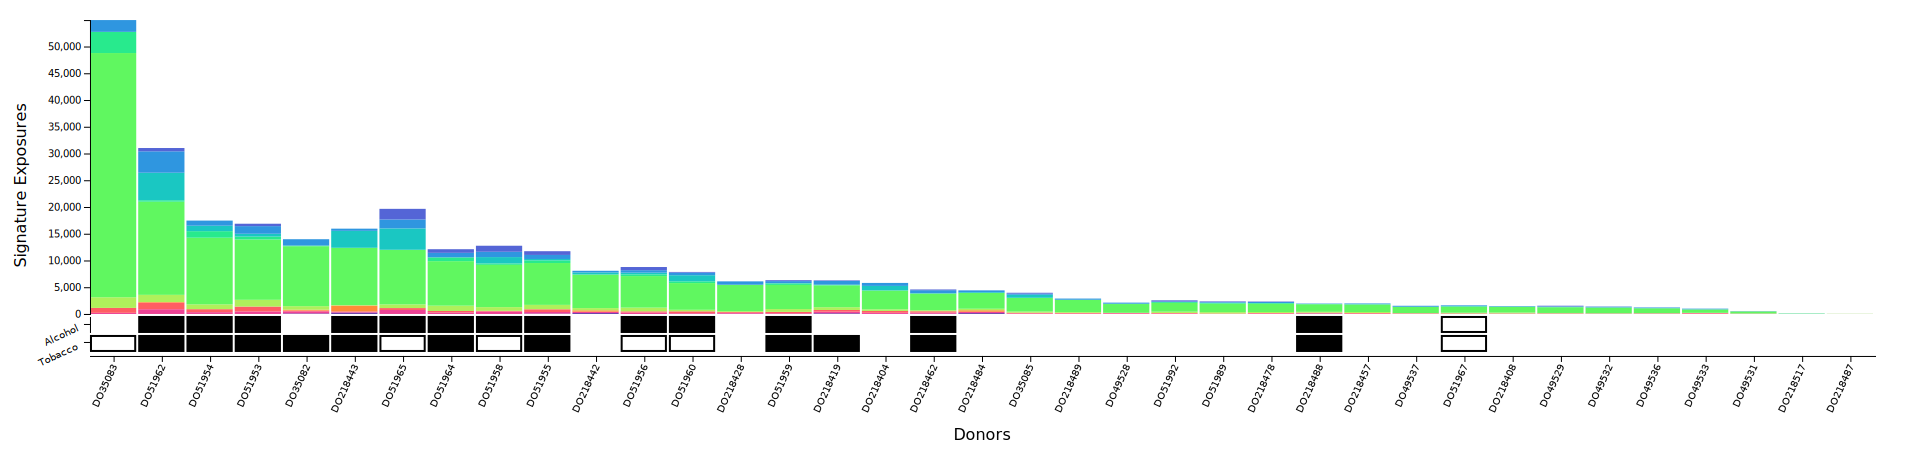
\includegraphics[width=\columnwidth]{figures/exposures.pdf}
\end{figure}
\begin{figure}[h!]
    \caption{Kataegis Plot (Chromosome 2)}
    \centering
    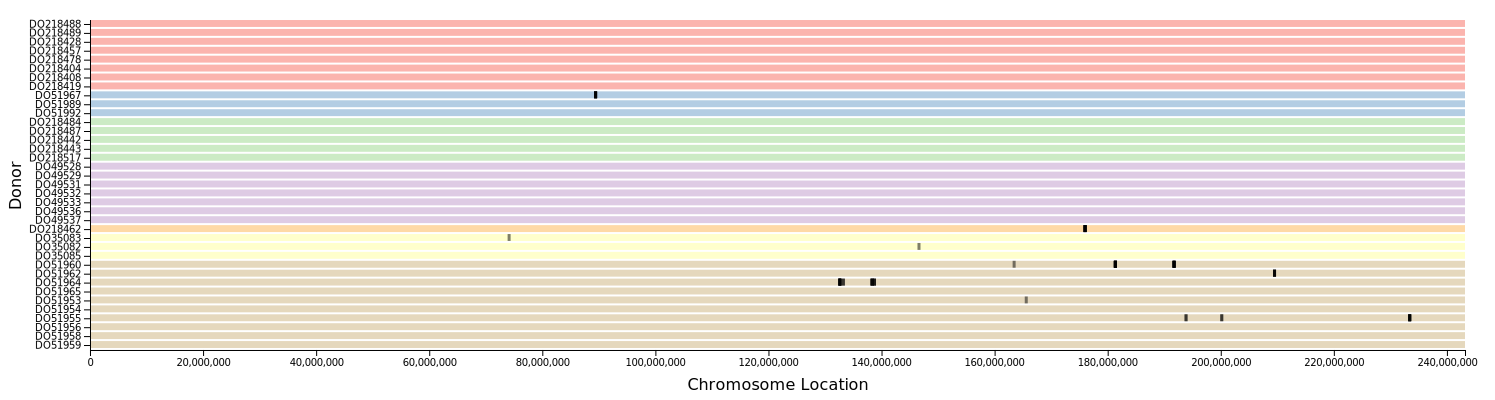
\includegraphics[width=\columnwidth]{figures/kataegis_chr2.pdf}
\end{figure}
\begin{figure}[h!]
    \caption{Rainfall Plot (Chromosome 6)}
    \centering
    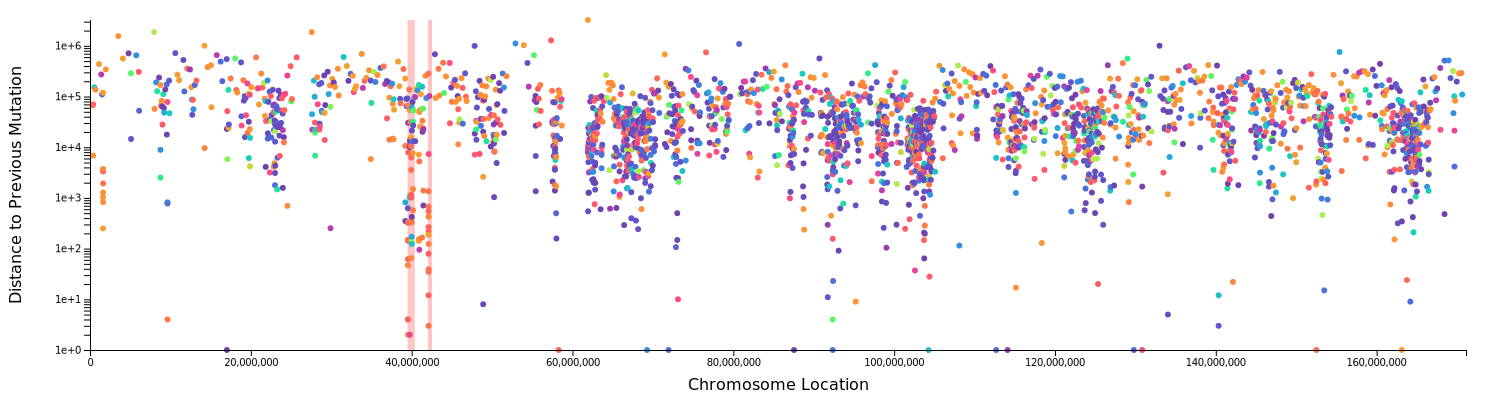
\includegraphics[width=\columnwidth]{figures/rainfall_DO50346_chr6.pdf}
\end{figure}
\begin{figure}[h!]
    \caption{Manhattan Plot (Chromosome 2)}
    \centering
    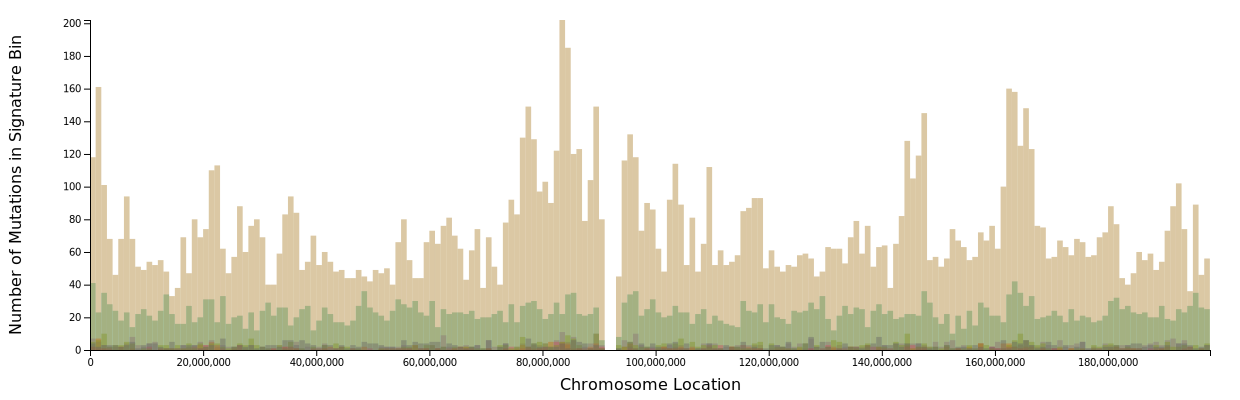
\includegraphics[width=\columnwidth]{figures/manhattan.pdf}
\end{figure}

\end{document}
